% Use dblanonrev for Double Anonymous Review submission
% Use sglanonrev for Single Anonymous Review submission
\documentclass[ijoc,sglanonrev]{informs4}
%\documentclass[ijoc,dblanonrev]{informs4}
\usepackage{eqndefns-left} % For checking the display equation width and equation environment definitions %
\RequirePackage{tgtermes}
\RequirePackage{newtxtext}
\RequirePackage{newtxmath}
\RequirePackage{bm}
\RequirePackage{endnotes}

%\OneAndAHalfSpacedXI
\OneAndAHalfSpacedXII % Current default line spacing
%%\DoubleSpacedXI
%%\DoubleSpacedXII

% Optional LaTeX Packages
\usepackage{url}
%\usepackage{graphicx}
\usepackage[T1]{fontenc}
\usepackage[algo2e,linesnumbered,ruled]{algorithm2e} 
%\usepackage{appendix}
\usepackage{tabularx}       % automatic column width
%\usepackage{subfig}        % two aligned subfigures
\usepackage{mathtools}  
\usepackage{amsfonts}       % mathbb
\usepackage{amsmath}        % aligned equations
\usepackage{xfrac}          % slanted fractions
\usepackage{bm}             % bold greeks 
\usepackage [autostyle, english = american]{csquotes} % left and right opening quotes with "
\usepackage{wrapfig}        % text flows around image
\usepackage{array}          % Needed for custom column types
\usepackage{xcolor}
\colorlet{added}{blue!80!black} 
%\usepackage{setspace}      % for controlled interline
%\usepackage{lineno}
\usepackage{enumitem}
\usepackage{tikz}           % drawing figures

\usepackage{caption}
\usepackage[labelfont=sf]{subcaption}
\captionsetup{subrefformat=parens,font=footnotesize}
\subcaptionsetup[figure]{textfont=sf,position=bottom}

\allowdisplaybreaks[4]
\interdisplaylinepenalty=100
\raggedbottom  % In preamble; allows uneven page bottoms

% Private macros here (check that there is no clash with the style)

% Natbib setup for author-number style
\usepackage{natbib}
 \bibpunct[, ]{(}{)}{,}{a}{}{,}%
 \def\bibfont{\small}%
 \def\bibsep{\smallskipamount}%
 \def\bibhang{24pt}%
 \def\newblock{\ }%
 \def\BIBand{and}%

%% Setup of the equation numbering system. Outcomment only one.
%% Preferred default is the first option.
\EquationsNumberedThrough    % Default: (1), (2), ...
%\EquationsNumberedBySection % (1.1), (1.2), ...

%% Setup of theorem styles. Outcomment only one.
%% Preferred default is the first option.
\TheoremsNumberedThrough     % Preferred (Theorem 1, Lemma 1, Theorem 2)
%\TheoremsNumberedByChapter  % (Theorem 1.1, Lema 1.1, Theorem 1.2)
\ECRepeatTheorems  %  

% For new submissions, leave this number blank.
% For revisions, input the manuscript number assigned by the on-line
% system along with a suffix ".Rx" where x is the revision number.
\MANUSCRIPTNO{IJOC-0001-2024.00}

% Redefine X column in tabularx to center the content
\newcolumntype{C}{>{\centering\arraybackslash}X}

%% the following for reducing space around figures
\setlength{\intextsep}{4pt}
\setlength{\textfloatsep}{4pt}
\setlength{\textfloatsep}{4.0pt plus 2.0pt minus 2.0pt}
%\captionsetup{belowskip=0pt}
\setlist[itemize]{noitemsep,nolistsep}

\MakeOuterQuote{"}
\def\UrlFont{\rmfamily}


%%%%%%%%%%%%%%%%
\begin{document}
%%%%%%%%%%%%%%%%
\let\WriteBookmarks\relax
\def\floatpagepagefraction{1}
\def\textpagefraction{.001}
	
% Reduce space before and after align
\setlength{\abovedisplayskip}{2pt plus 2pt minus 4pt}
\setlength{\belowdisplayskip}{2pt plus 2pt minus 4pt}
\setlength{\abovedisplayshortskip}{0pt}
\setlength{\belowdisplayshortskip}{0pt}

% Outcomment only when entries are known. Otherwise leave as is and
%   default values will be used.
%\setcounter{page}{1}
%\VOLUME{00}%
%\NO{0}%
%\MONTH{Xxxxx}% (month or a similar seasonal id)
%\YEAR{0000}% e.g., 2005
%\FIRSTPAGE{000}%
%\LASTPAGE{000}%
%\SHORTYEAR{00}% shortened year (two-digit)
%\ISSUE{0000} %
%\LONGFIRSTPAGE{0001} %
%\DOI{10.1287/xxxx.0000.0000}%

% Author's names for the running heads
\RUNAUTHOR{Fenga and Maniezzo}

% Title or shortened title suitable for running heads. Sample:
\RUNTITLE{BESO for 2-echelon logistics}

% Full title. Sample:
\TITLE{Bootstrap Enhanced Scenario Optimization, a Case Study in Two-Echelon Logistics}

% Block of authors and their affiliations starts here:
\ARTICLEAUTHORS{%
\AUTHOR{Livio Fenga}
\AFF{Center for Simulation, Analytics and Modelling,
University of Exeter, \EMAIL{L.Fenga@exeter.ac.uk}}

\AUTHOR{Vittorio Maniezzo}
\AFF{Department of Computer Science,
University of Bologna, \EMAIL{vittorio.maniezzo@unibo.it}}
} % end of the block

\ABSTRACT{
We introduce the Bootstrap Enhanced Scenario Optimization (BESO) framework, a novel methodology for prescriptive analytics under uncertainty. BESO addresses the challenge of generating reliable demand scenarios from volatile, short, and non-stationary time series data. The core innovation lies in delegating the modeling of uncertainties to the Maximum Entropy Bootstrap (MEB) integrated with bagging, a technique that preserves the complex autocorrelation structure of empirical time series forecasts, enabling the generation of statistically coherent scenarios. We further extend MEB through an objective-augmented formulation that incorporates downstream recourse elements into the resampling mechanism. These statistically rich scenarios are then integrated into a deterministic equivalent model to derive accountable and optimized prescriptions. We demonstrate the framework's power using a real-world case study in tactical inventory allocation. Our findings, also validated against an extensive set of artificial benchmark instances, demonstrate the effectiveness of MEB-enhanced forecasting in optimization. BESO establishes a new, generalizable paradigm for robust decision-making derived from noisy univariate data series.
}%

%\FUNDING{This research was supported by [grant number, funding agency].}

%Supplemental Material:
%Data Ethics & Reproducibility Note:

% Fill in data. If unknown, outcomment the field
\KEYWORDS{Stochastic programming, Distributionally Robust Optimization, Forecasting, Maximum Entropy Bootstrap, Two-echelon logistics} 
%\HISTORY{Received: Month DD, YYYY; Accepted: Month DD, YYYY; Published Online: Month DD, YYYY}

\maketitle
%%%%%%%%%%%%%%%%%%%%%%%%%%%%%%%%%%%%%%%%%%%%%%%%%%%%%%%%%%%%%%%%%%%%%%

\section{Introduction} \label{Sec:intro}

Decision-making under uncertainty is a pervasive challenge in operations research, particularly in complex systems such as logistics networks. Scenario-based optimization has long been used to address this challenge by capturing the variability of future events through a finite set of possible outcomes. However, the reliability of such methods depends heavily on how accurately these scenarios represent the underlying stochastic processes.

In this paper, we propose a novel method —- {\em Bootstrap Enhanced Scenario Optimization} (BESO) —- that integrates bootstrap-based forecasting with scenario-based linear optimization to enhance the robustness and realism of stochastic modeling. The approach can be framed within the Distributionally Robust Optimization (DRO) paradigm; however, unlike mainstream moment- or ambiguity-set-based formulations, it leverages statistical models fitted to empirical data to generate optimization-ready scenarios.

BESO introduces a twofold, decision-aware extension of the Maximum Entropy Bootstrap (MEB). First, the bootstrap objective is augmented with optimization cost components, allowing scenario generation to internalize downstream decision criteria. Second, we explicitly account for the effect of bootstrap-set cardinality on the resulting optimization outcomes, recognizing scenario size as a structural parameter shaping the effective ambiguity set. Together, these mechanisms create a feedback loop between the optimization model and the statistical resampling phase: the ambiguity set remains statistically coherent while its geometry and dispersion are partially shaped by optimization-relevant considerations. The framework is particularly suited to predictive settings where reliable historical time series are available.

The resulting data-driven methodology for empirically estimating the distribution of stochastic variables and embedding it in scenario generation for robust and stochastic optimization may offer significant advantages over standard distribution-aware approaches. Traditional methods often rely on strong assumptions about the underlying probability distribution — typically normality or other parametric forms — which may not accurately reflect the true behavior of real-world uncertainties. In contrast, data-driven techniques directly leverage historical or observed data to construct empirical distributions, capturing nuances such as asymmetry, multimodality, or heavy tails that standard models might overlook. This increased fidelity can lead to more realistic and effective scenario generation, improving both the robustness and relevance of the resulting optimization solutions. Furthermore, by adapting to the structure present in the data, data-driven approaches are naturally more flexible and can better accommodate nonstationarities or structural changes in the stochastic environment, providing better alignment with real operational environments.

To demonstrate the practical value and performance of BESO, we apply it to a real-world two-echelon logistics network problem. In this setting, uncertain outbound freight demands must be satisfied across multiple depots. By using BESO to define demand scenarios and solve for optimal allocation decisions and related inventory requests, we show how the method improves the solution robustness compared to conventional techniques, while remaining conceptually transparent, computationally efficient and straightforward to implement.

%The remainder of the paper is structured as follows: Section \ref{Sec:literature} reviews previous works related to the different research areas intersected by this study. Section \ref{Sec:testcase} describes the case study that motivated our research. Section \ref{Sec:forecasting} and \ref{Sec:optimization} present the BESO methodology in detail.  Section \ref{Sec:results} discusses the computational results, and Section \ref{Sec:conclusions} concludes with key insights and future research directions.

\section{Literature review} \label{Sec:literature}

The paper intersects different research threads, both in terms of the theoretical contribution and the application use case.

\subsection{Predictive Prescriptions and Distributionally Robust Optimization}

Stochastic programming has long served as a fundamental framework for modeling decision-making under uncertainty, primarily through expected-value models and recourse formulations \citep{D55,B55}. As the field matured, methods evolved to address model robustness. Robust optimization \citep{BS04} proposes a deterministic reformulation considering worst-case outcomes within a defined uncertainty set. A major development is {\it Distributionally Robust Optimization} (DRO), which seeks a solution most resilient against the worst-case probability distribution for uncertain parameters, typically within an {\it ambiguity set} \citep{DY10}.

The ambiguity set ($\mathcal{U}$) in DRO is a carefully constructed set of probability distributions that the true, but unknown, distribution of the uncertain parameters is assumed to belong to. The core of DRO is to optimize the worst-case performance over all distributions within this set, thus making the resulting solution robust to distributional uncertainty. Mainstream DRO approaches define this ambiguity set in different ways. Some utilize specific distance metrics to construct an ambiguity set centered around the empirical distribution, such as those based on the $\phi$-divergence (or $f$-divergence) \citep{BK19}. Others, such as in the work of \citet{EK17}, define the set based on measurable moment constraints (e.g., bounds on the mean and covariance) of the uncertain parameters. This methodology provides strong theoretical guarantees but requires the designer to make choices on the ambiguity set's structure and size, which may not fully reflect the true statistical dynamics of the input data.

A primary technique for applying both stochastic programming and DRO is {\it Scenario-Based Optimization}. This approach discretizes the continuous probability distribution of uncertain parameters into a finite set of specific scenarios. The {\it Sample Average Approximation} (SAA) method is a pivotal technique here \citep{SH98}, approximating the true underlying distribution with an empirical distribution derived from a sample of independent and identically distributed realizations.

The integration of forecasting and scenario-based optimization - often framed as {\it predict-then-optimize} - is a growing body of literature \citep{BK19}. The typical workflow follows a two-stage paradigm: a forecasting model (e.g., SARIMA, GARCH, LSTM) first estimates future parameters, and a separate scenario generation phase simulates or samples future paths based on the forecast's predictive distribution. This sequential paradigm has been questioned because prediction errors, even small ones, can lead to suboptimal decisions when their impact on the downstream optimization problem is large. This motivated the development of methods that explicitly incorporate the optimization objective into the forecasting model's loss function \citep{DAK17}, leading to the "Smart Predict, then Optimize" (SPO) framework \citep{EG22}, besides the aforementioned DRO contributions.

Unlike these traditional DRO and predict-then-optimize approaches, our work introduces a novel framework that fundamentally links the statistical modeling of input data to the generation of the uncertainty set. Our {\it Bootstrap Enhanced Scenario Optimization} (BESO) framework leverages bootstrapped time series to generate future scenarios. This approach is conceptually aligned with DRO, as it seeks robustness across a set of statistically plausible distributions. However, by using the Maximum Entropy Bootstrap (MEB), BESO generates scenarios that directly preserve the complex autocorrelation and non-stationarity observed in the historical data, eliminating the need for post-hoc parametric ambiguity set design. Scenarios are not a post-processing step but emerge directly from a statistically robust model of the input data's empirical structure. Furthermore, we show how the MEB objective function can be extended to incorporate the downstream optimization's recourse objective, thereby aligning the statistical model directly with the desired prescriptive outcome, similar to SPO methods. In addition, the bootstrap-set cardinality acts as an explicit structural control on the induced ambiguity, allowing the dispersion and effective geometry of the scenario set to be tuned in accordance with downstream optimization sensitivity.

\subsection{2-echelon logistics networks}

Multi-echelon inventory management is a supply chain control strategy that coordinates inventory across multiple levels, called "echelons," of the chain \citep{Clark60}. The objective is to optimize inventory and routing costs across all levels of the supply chain rather than addressing each level in isolation. The literature on this strategy has expanded significantly, covering various aspects such as inventory control policies, replenishment strategies, and inventory risk management.

The successful implementation of effective management policies hinges on sound forecasting and optimization processes. Specifically, in the context of 2-echelon logistics, prescriptions grounded in predictive analytics are essential for refining demand forecasting, inventory allocation, and transportation planning \citep{A01}. Considerable attention has been paid to demand forecasting \citep{Ma15,Shenstone01}, however, precise demand forecasting, especially within the context of dynamic retail environments characterized by fluctuating trends and seasonal variations, remains a significant obstacle. Multi-echelon demand forecasting commonly incorporates a variety of models that frequently rely on assumptions of stationarity and specific parametric distributional characteristics that are often violated in dynamic retail environments characterized by short-horizon, non-stationary demand series, leading to model mismatch and suboptimal prescriptions.

The application of prescriptive analytics in 2-echelon logistics systems thus faces a critical challenge: how to robustly model the underlying uncertainty to support efficient management decision processes. Most documented multi-echelon inventory policies in the literature rely on instances with generic demand, often generated according to parametric distributions \citep{Escorcia20}. Our work addresses this methodological gap.

By introducing the BESO framework, we provide a statistically-grounded approach to tactical logistics planning. BESO leverages the MEB to generate demand scenarios that accurately preserve the complex autocorrelation and non-stationary structure of empirical demand data. This novel method directly counters the limitations of traditional approaches that fail to capture the nuances of real-world volatility, enabling the distribution centers (DCs) to update their market forecast and anticipate the structural attributes of the model, ultimately providing valuable management insights \citep{P16}. We demonstrate this capability using a comprehensive real-world case study where all instance elements, from demand series to network configurations, are derived from actual records. This application provides a validation of how BESO improves both solution robustness and operational efficiency in multi-echelon inventory management.

\section{The 2-echelon test case} \label{Sec:testcase}

The test case, that makes use of data that comes from an LSRT company that manages multiple retail stores in a large city in northern Italy, originally proposed in \citet{MZ23} for a different application. In this case, 52 stores provided aggregate sales time series data spanning at least 45 months prior to the forecast period, which is set at a three-month horizon, as detailed in the following. Each store maintains a small inventory, replenished by deliveries from one of four different distribution centers (DCs) in the area. The products are categorized into three lines: fresh, dry, and household. In this context, the focus has been exclusively on the logistics of dry and household goods, including product categories ranging from personal care items to basic electronics, from household goods to holiday decorations. For this product line, DCs are required to maintain an aggregate inventory sufficient to cover a demand for a period of two weeks.

The supply chain consists of a large distribution center (DC) in the northern suburbs of the city, a smaller DC in the south, and two small satellite facilities closer to the city center. The satellites have limited storage capacity, but they offer lower-cost and more timely service to the majority of the city's stores. 
Each store must be allocated to a distribution center (DC), ensuring that the total requests made to a DC do not exceed its storage capacity. It is assumed that the handling and transportation capacities will always be sufficient. Both storage capacities and requests are quantified in terms of pallets, with no further granularity at this level. The cost of servicing a store from a DC is assessed based on the travel time required to transport goods between the two entities. Notably, the three smaller DCs are owned by the company, whereas the fourth DC is situated in a leased facility.

The ultimate goal of the analysis is to determine how much space to rent during the next peak demand period, the Christmas season. To achieve this, we first optimize the allocation of stores to DCs, taking into account transportation and storage costs, and from the solution it is immediate to derive the space required in each DC, therefore the space to rent in the largest one.

Another requirement characterizes the problem we are addressing: large stores located near small DCs often lead to rapid saturation of the capacity of central DCs. This forces nearby stores to be served by comparatively distant DCs. Therefore, it has been proposed to allow tentative split service for certain selected stores to facilitate what-if analysis. The problem we address thus involves a parametric number of possible assignments for each store, where which store should be allowed multiple (double) assignments is an input parameter, not a decision variable.  

The analysis was conducted during the summer of 2022 in preparation for the subsequent Christmas season. At the time of the analysis, the anticipated demand requests were unknown and required forecasting. The analysis underwent iterative refinements throughout the summer, culminating in the final forecast produced in September. Consequently, the data presented in this paper correspond to a three-month forecasting case. 

All codes and data are available in an anonymized format from the project repository 
%\citep{GDOforecastRepo}
{\it (public upon acceptance)}. Specifically, the file containing the request time series can be downloaded from the repository, where all series are complete up to the most recent actual values. However, it should be noted that the last three values were unknown at the time the final forecast was generated. 

\section{The predictive module} \label{Sec:forecasting}

Data-driven approaches to estimating the distribution of stochastic variables have gained increasing attention as alternatives to classical parametric modeling, particularly in settings where assumptions of stationarity or known distributional forms are invalid. Unlike traditional techniques that rely on a priori specification of distribution families (e.g., Gaussian or Poisson), data-driven methods infer distributional characteristics directly from historical or observed data, making them especially suited for real-world applications with complex, noisy, or limited information.

Among the most prominent techniques are resampling-based methods such as the Bootstrap \citep{b1}, which generates empirical distributions by repeatedly sampling from the data with replacement. The Maximum Entropy Bootstrap (MEB) \citep{Vinod2006} extends this idea by producing replicates that preserve dependence structures in time series data, making it particularly valuable for short or non-stationary sequences.

Recent work has explored the integration of these empirical distribution estimates into stochastic and robust optimization pipelines. Notable contributions include nonparametric scenario generation \citep{BM11}, distributionally robust optimization using empirical Wasserstein distances \citep{EK17}. 

In our proposal, we utilize the MEB methodology in conjunction with the ensemble learning technique known as {\it bagging} (Bootstrap Aggregating). This combination enhances the accuracy and robustness of predictive models through the generation of multiple bootstrapped datasets from the original data. By training individual models on these datasets and aggregating their predictions through averaging, we adhere to MEB's principles while capturing the underlying statistical variability. Maximizing entropy under empirical constraints allows the integration of bagging with MEB to produce more robust models. In more details, each model trained on distinct bootstrapped samples incorporates uncertainty characteristics from the original data, allowing for a comprehensive representation of its variation.

Furthermore, this approach allows for dealing with noisy datasets and mitigating overfitting, as bagging inherently provides a mechanism to increase the robustness of the predictive model by leveraging the diversity across the bootstrapped samples. Since MEB generates bootstrapped datasets based on the maximum entropy principle, the resulting models avoid being overly sensitive to any one particular realization of the data.

%Mathematically, if we denote the bootstrapped replicas of the dataset as $D^*_1, D^*_2, \ldots, D^*_B$, where $B$  represents the number of bootstrapped samples, the resulting predictive framework can be expressed as:  $\hat{y}_{\textit{BAG}} = \rho( \hat{y}_{b}(x) )$, where $\hat{y}_{b}(x)$ is the prediction made by the $b-th$ model trained on the bootstrapped sample $ D^*_b $  and $\rho$ a generic centrality parameter. 
%This averaging process effectively reduces variance by smoothing out the predictions of the individual models, leading to enhanced stability and generalization capabilities in the final aggregated model.  The parameter $\rho$ can be defined as either a simple average or the median, which leads to the following bagging predictors, where, $\hat{y}_{b}(x)$  is  sorted in ascending order whereas $h$ is the number of future values to be predicted.
%\begin{align}
%	\hat{y}_{\textit{BAG}} &= \frac{1}{B} \sum_{b=1}^{B} \hat{y}_{b}(x) &
%	\hat{y}_{\textit{BAG}} &=
%	\begin{cases}
%		\hat{y}_{b}(x)\left[\frac{h+1}{2}\right] & \text{if } h \text{ is odd} \\
%		\frac{\hat{y}_{b}(x)\left[\frac{h}{2}\right] + \hat{y}_{b}(x)\left[\frac{h}{2} + 1\right]}{2} & \text{if } h \text{ is even}
%	\end{cases}
%\end{align}

\subsection{Resampling techniques} \label{Subsec:resampling}

In recent years, bootstrap resampling has become a valuable tool for overcoming limitations of conventional forecasting methods \citep{hasni2019spare}. By generating simulated time series from observed data, it 
%is particularly effective for non-stationary, non-linear, and low signal-to-noise settings \citep{kreiss2012bootstrap}. It also
helps mitigating issues related to small sample sizes \citep{davison1997bootstrap} and model uncertainty \citep{sarris2020exploiting}.
Bootstrap methods have also proven effective in model selection. \citet{fenga2011bootstrap} proposed a bootstrap-based approach for ARMA order selection, improving accuracy in finite samples, and for high-dimensional sparse autoregression \citep{fenga2017lasso}, highlighting the relevance of bootstrap techniques in modern statistical modeling.

However, standard bootstrap assumes independent and identically distributed (i.i.d.) data, which is inappropriate for time series characterized by dependence, autocorrelation, and structural patterns. This limitation is particularly critical for short series, where resampling can distort temporal structure and underestimate variability. In this context, Maximum Entropy Bootstrap (MEB) provides several advantages, including 
$i$) {\it Preservation of dependence structure}: maintains autocorrelation, trend, and seasonality through rank-based reordering and interpolation;
$ii$)  {\it Suitability for short series}: preserves local features and generates plausible data paths under limited observations; 
$iii$)  {\it Model-free approach}: avoids parametric assumptions and tuning choices such as block length or ARMA specification; 
$iv$)  {\it Smooth pseudo-series generation}: produces continuous series suitable for inference and forecasting; 
$v$)  {\it Maximum entropy principle}: generates least-biased samples consistent with observed data; 
$vi$)  {\it Flexibility}: applicable to both stationary and non-stationary series.

The MEB framework builds on the {\it Maximum Entropy Principle} (MEP) \citep{shannon1948mathematical}, which selects the probability distribution that maximizes uncertainty subject to known constraints \citep{jaynes1957information}. This is formalized via Shannon entropy, $S(p) = -\sum_{i=1}^{n} p_i \log(p_i)$, where $p_i$ denotes the probability of the $i$-th outcome in a sample space of size $n$.

The pivotal advancement provided by MEB lies in its ability to formulate bootstrapped samples that adhere to a spectrum of constraints dictated by the original dataset, such as predetermined moments, probabilities, or other statistical characteristics \citep{berger1985statistical}. These constraints can be specified in the form of normalized probabilities and empirical expectations, expressed as $\sum_{i=1}^{n} p_i = 1$ to ensure that the probabilities form a valid distribution, and $\sum_{i=1}^{n} p_i f_i = \bar{f}$, where $f_i$ represents measurements or statistics relevant to the analysis, with $\bar{f}$ being the empirical mean of these measurements. The formulation of the Maximum Entropy problem consequently leads to a constrained optimization framework. The optimization problem can be succinctly encapsulated in the Lagrangian:
\begin{equation}
	L(p, \lambda, \mu) = S(p) + \lambda \left(1 - \sum_{i=1}^{n} p_i\right) + \mu \left(\bar{f} - \sum_{i=1}^{n} p_i f_i\right),
\end{equation}
where $\lambda$ and $\mu$ are Lagrange multipliers that adjust the balance under the constraints of normalizing the distribution and matching the empirical mean, respectively. The solution to this maximization problem yields a probability distribution, which appears as
$p_i = \frac{e^{\mu f_i}}{\sum_{j=1}^{n} e^{\mu f_j}}$,  where the parameter $\mu$ is determined through the constraint equations, specifically via a numerical root-finding approach that satisfies the moment condition $\sum_{i=1}^{n} p_i f_i = \bar{f}$.

Building on this classical formulation, we define an Objective-Augmented Maximum Entropy Bootstrap (OA-MEB) scheme that incorporates additional optimization-oriented structure directly into the resampling distribution. To do so, we introduce an auxiliary objective-related component $g_i$, representing scenario-wise quantities that are relevant to downstream decision or cost functions in stochastic programming (e.g., expected cost contributions, constraint violations, or risk-sensitive statistics). The OA-MEB extends the entropy maximization problem by embedding a tunable scalar parameter $\gamma \ge 0$ that controls the influence of this additional term while preserving the probabilistic and moment-matching constraints. The resulting augmented Lagrangian is given by:
\begin{equation}
	L_{\mathrm{OA}}(p, \lambda, \mu, \gamma) = S(p) 
	+ \lambda \left( 1 - \sum_{i=1}^{n} p_i \right)
	+ \mu \left( \bar{f} - \sum_{i=1}^{n} p_i f_i \right)
	+ \gamma \left( \sum_{i=1}^{n} p_i g_i \right),
\end{equation}
where the additional inner product term $\sum_{i=1}^{n} p_i g_i$ promotes bootstrap resamples that remain statistically coherent while incorporating optimization-driven scenario emphasis. Solving the first-order optimality conditions yields a modified exponential-tilting solution: 
$
	p_i^{\mathrm{OA}} = \frac{\exp\left(\mu f_i + \gamma g_i\right)}
	{\sum_{j=1}^{n} \exp\left(\mu f_j + \gamma g_j\right)},
$, showing that classical MEB is recovered as the special case $\gamma = 0$. Calibration of $\gamma$ governs the trade-off between purely information-theoretic sampling and decision-aligned resampling, and may be performed via cross-validation, bilevel optimization, or risk-preference calibration strategies consistent with the downstream stochastic programming model.

This formulation transforms the problem into one that allows for flexible adaptation to various types of data and constraints imposed by the empirical observations. Once this extended maximum entropy distribution is established, resampling via bootstrapping can be accomplished by selecting  $m$ samples according to the derived $p_i$.  This produces synthetic datasets that not only reflect the variability and uncertainty characteristic of the original data but also adhere to the specific constraints imposed, which may include higher moments or even domain-specific statistics. 

This resampling process can be iterated to generate a comprehensive set of bootstrapped samples, enabling a multitude of statistical analyses, including confidence interval estimation, hypothesis testing, and model validation \citep{efron1993introduction}. 

\subsection{Bootstrap Cardinality and Decision--Ambiguity Feedback} \label{Subsec:ambiguity}

Bootstrap-based ambiguity sets introduce an additional degree of freedom in data-driven DRO: the bootstrap cardinality $m$. Although often treated as a tuning parameter, $m$ directly determines the geometry of the ambiguity set and therefore influences the optimizer. Conversely, the optimal decision induces a preference over $m$ through validation or penalization criteria. This creates an intrinsic feedback loop between ambiguity construction and optimization, which the MEB-extension formalizes.
We observe data $D_n=\{\xi_i\}_{i=1}^n$ with empirical measure
$\widehat{P}n=\frac{1}{n}\sum{i=1}^n \delta_{\xi_i}$, decision space $X\subset\mathbb{R}^d$, and cost function $c:X\times\Xi\to\mathbb{R}$.  
For a bootstrap scheme, let $\widehat{P}_n^{(1)},\dots,\widehat{P}_n^{(m)}$ denote $m$ bootstrap empirical measures.  
A natural ambiguity set is the convex hull
$\mathcal{U}_m := \operatorname{conv}\{\widehat{P}_n^{(1)},\dots,\widehat{P}_n^{(m)}\}$	
where $\widehat{P}_n^{(j)}$ is the empirical distribution of the (j)-th bootstrap sample, and $\mathcal U_m$ is their convex hull in the space of measures whose diameter, extreme points, and support all depend on $m$.
The associated DRO objective is $\Psi_m(x) := \sup_{P\in\mathcal{U}_m} \mathbb{E}_P[c(x,\xi)],
$ and the optimizer is defined by $x^\star(m)\in\arg\min_{x\in X}\Psi_m(x)$.

Since $\Psi_m$ is the supremum of finitely many linear functionals $\mathbb{E}_{\widehat{P}_n^{(j)}}[c(x,\xi)]$, changing $m$ changes the set of extreme points and therefore the optimizer. In general, $m\neq m'$ implies $\mathcal{U}_m\neq\mathcal{U}_{m'}$ and $x^\star(m)\neq x^\star(m')$.
If the ambiguity set depends on $x$—for example through residual-based resampling in the MEB-extension—write $\mathcal{U}_m(x)$ and consider the joint problem
\begin{equation}
	\min_{x\in X,\; m\in\mathcal{M}}
	\left\{
	\sup_{P\in\mathcal{U}_m(x)} \mathbb{E}_P[c(x,\xi)]
	+ \lambda\,\mathrm{Pen}(m)
	\right\}.
\end{equation}
Eliminating $m$ yields the bilevel formulation
\begin{equation}
	\min_{m\in\mathcal{M}} 
	\Phi(x^\star(m),m)
	\quad\text{s.t.}\quad
	x^\star(m)\in\arg\min_{x\in X}
	\sup_{P\in\mathcal{U}_m(x)}\mathbb{E}_P[c(x,\xi)].
\end{equation}
This expresses the feedback loop: $m$ shapes the ambiguity faced by $x$, while $x$ determines which $m$ minimizes the joint objective.
Under standard bootstrap consistency assumptions, if $m=m(n)\to\infty$ with $m(n)/n\to 0$, then $\mathcal{U}{m(n)}\Rightarrow P^\star$ and $\Psi{m(n)}(x)\to\mathbb{E}_{P^\star}[c(x,\xi)]$ uniformly on compact $X$, implying $x^\star(m(n))\to x^\star$. For finite $n$,
\begin{equation}
	\sup_{x\in X}\big|\Psi_m(x)-\Psi_{m'}(x)\big|
	\le 
	L\,\mathrm{Haus}\!\left(\mathcal{U}m,\mathcal{U}{m'}\right),
\end{equation}
so changes in $m$ induce controlled perturbations in the DRO objective and optimizer.

The MEB-extension incorporates decision-dependent ambiguity and regularizes $m$ within the joint objective, replacing the classical ``forecast--then--optimize'' pipeline with a unified formulation that captures the $m\leftrightarrow x^\star(m)$ feedback.

%\begin{figure}[h!]
%	\centering
%	\begin{tikzpicture}[>=stealth,thick]
	%		
	%		% Nodes (no line breaks inside nodes)
	%		\node[draw,rounded corners,align=center] (m) at (0,0)
	%		{$m$ \text{ (bootstrap cardinality)}};
	%		
	%		\node[draw,rounded corners,align=center] (U) at (4,0)
	%		{$\mathcal{U}_m$ \text{ (ambiguity set)}};
	%		
	%		\node[draw,rounded corners,align=center] (x) at (8,0)
	%		{$x^\star(m)$ \text{ (DRO optimizer)}};
	%		
	%		% Arrows
	%		\draw[->] (m) -- node[above]{shapes} (U);
	%		\draw[->] (U) -- node[above]{defines} (x);
	%		\draw[->,bend left=35] (x.north) to node[above]{selects $m$ minimizing $\Phi$} (m.north);
	%		
	%	\end{tikzpicture}
%	\caption{Feedback loop between bootstrap cardinality $m$, ambiguity geometry $\mathcal{U}_m$, and the DRO optimizer $x^\star(m)$.}
%\end{figure}

\section{The prescriptive module} \label{Sec:optimization}

The predictive module provides a structural component of the prescriptive module, which aims to optimize the allocation of stores to distribution centers (DCs), thereby enabling the quantification of space to rent in third-party DCs. The results of the optimization are in turn used to evaluate the modeled {\it scenario}, where scenarios are defined for specific what-if analyses. For example, the objective of the what-if analyses could be to examine the effect of freezing some allocations while leaving free the others, or possibly accepting some multiple -- double in the test case -- allocations for some selected stores. 

The core optimization problem is a {\em split allocation problem}. This variant of the basic allocation problem has already received attention in the optimization literature, mainly in the context of survivable communication network design \citep{MKE75}, and more generally as the splittable capacitated multiple allocation hub location problems \citep{M05}. It finds applications in fiber optic access networks \citep{KLH11}, split delivery routing \citep{DT89}, and even in school timetabling \citet{BBL07}. The problem we are interested in is related to one that is presented in \citet{ZHHY21}, but it is modelled in a very different way.
The mathematical model we use is a direct extension of the standard model for allocation problems. As our proposed framework is valid beyond the specific case study described in the paper, we will refer to the application elements (stores and data centers) using standard allocation terminology in what follows. To emphasize the generality of the analysis, we will use the more generic term 'clients' to denote the stores and 'servers' to denote the centers. In our context, the constraints can accept a parametric number of assignments, enabling requests to be serviced across multiple servers. 
\begin{align}
	&(FD) & z_{FD} = \textbf{min } & \sum_{i \in I} \sum_{j \in J} ( c_{ij}x_{ij} + d_i q_{ij} ) \label{ALLobj}\\
	& &  \textbf{subject to }
	& \sum_{i \in I} q_{ij} = req_j & j \in J  \label{ALLrequest}\\
	& &  & \sum_{j \in J}q_{ij} \leq Q_i & i \in I \label{ALLcapacity}\\
	& &  & \sum_{i \in I} x_{ij} = b_j & j \in J  \label{ALLnumserv}\\
	& &  & q_{ij} \leq req_j x_{ij}; \quad x_{ij} \in \{0,1\};\quad q_{ij} \in \mathbb{Z}^+_0 & i \in I, j \in J \label{ALLcontin}
\end{align}
The notation used in the model is as follows:
	$n$: number of clients (stores),
	$J$: index set of clients, $J=\{1, \ldots, n\}$,
	$m$: number of servers (DCs),
	$I$: index set of servers, $I=\{1, \ldots, m\}$,
	$c_{ij}$: global cost for allocating client $j \in J$ to server $i \in I$,
	$Q_i$: storage capacity of server $i \in I$,
	$d_i$: unit storage cost of server $i \in I$,
	$req_j$: total request of client $j$,
	$b_j$: maximum number of servers (DCs) client $j$ can be assigned to,
	$x_{ij}$: binary decision variable equal to 1 iff client $j$ is allocated to server $i$, $i \in I$ and $j \in J$,
	$q_{ij}$: integer decision variable representing the amount (number of pallets) of request of client $j$ provided from server $i$.
In the final test case, the amount requested by each client was always set to equal the corresponding predicted value. However, in some scenarios, some clients' requests could be split between two servers, meaning the requested $q_(ij)$ amounts could vary.
The mathematical model used for this problem is as in formulation (FD).

{\clubpenalty=50 \widowpenalty=50
The constraints in equation \ref{ALLnumserv} are formulated as equalities due to the need to impose specific splits in 'what if' scenarios. However, if this is not of particular interest, these constraints could be replaced by less-than-or-equal-to inequalities combined with inequalities that ensure allocations are made to at least one server.
Note that when $b_j = 1$ for all clients, i.e., when each client $j \in J$ can be served by only one server, constraints \ref{ALLcontin} and \ref{ALLrequest} force the entire quantity requested by client $j$, $req_j$, to be supplied by a single server. The constraints \ref{ALLcontin} thus become equations, the constraints \ref{ALLrequest} become redundant, and the constraints \ref{ALLcapacity} can be expressed by replacing $\sum_{j \in J}q_{ij}$ with $\sum_{j \in J}req_j x_{ij}$. Problem P reduces to the standard GAP and can be solved by any of the methods described in \citet{matheuristics}.
}
However, we are interested in the general case that allows for multiple assignments. Since the cost is derived from these assignments, the problem can be considered a fixed-cost split-assignment allocation problem.
Furthermore, as future client requests can only be forecast, it is more convenient to formulate the problem as a stochastic optimization problem, where the future requests are random variables $\rho_j$, $j \in J$, whose distributions are derived from the forecast results. The resulting stochastic problem is formulated as in formulation (FS), where the values $R(\rho_j)$ in the constraints \ref{SALLrequest} and \ref{SALLcontin} refer to any same realization of the random variable $\rho_j$.
\begin{align}
	&(FS) & z_{FS} = \textbf{min } & \sum_{i \in I} \sum_{j \in J} ( c_{ij}x_{ij} + d_i q_{ij} ) \label{SALLobj}\\
	& &  \textbf{subject to }
	& \sum_{i \in I} q_{ij} = R(\rho_j) & j \in J  \label{SALLrequest}\\
	& &  & \sum_{j \in J}q_{ij} \leq Q_i & i \in I \label{SALLcapacity}\\
	& &  & \sum_{i \in I} x_{ij} = b_j & j \in J  \label{SALLnumserv}\\
	& &  & q_{ij} \leq R(\rho_j) x_{ij}; \quad  x_{ij} \in \{0,1\}; \quad q_{ij} \in \mathbb{Z}^+_0 & i \in I, j \in J \label{SALLcontin}
\end{align}
Different methods can be used to deal with this case \citep{SDR09}. We transformed the formulation (FS) into its {\it deterministic equivalent} \citep{D55} using the forecasts computed on the bootstrap sets. We generated multiple scenarios each containing a realization of the stochastic variable $\rho$, which is defined as a forecast of one series from the bootstrap set in use. For each scenario $s$, we thus created a version of the constraint with $b_i^{s}$ as the right-hand side. The final solution must satisfy these constraints across all scenarios.
The objective function now incorporates the quantities to be delivered to each client in different scenarios. Therefore, we consider the expected cost as a weighted average across these scenarios and include it in the objective function. 
The resulting formulation is in formulation (DE). The random variables $\rho_j$ are sampled in a finite number of scenarios. Let $\rho^s_j$ denote the realization of $\rho_j$ in scenario $s$, $s \in S$, and let $p_s = \frac{1}{|S|}$ be the probability associated with scenario $s \in S$. The variables $\epsilon_{js}$ are slack variables for the customer service constraints.
\begin{align}
	&(DE)\quad z_{DE} = & \textbf{min} &\sum_{s \in S} \left( p_s \sum_{j \in J} \left( \sum_{i \in I} ( c_{ij}x_{ij} + d_i q_{ij}^s) + M \epsilon_{js} \right) \right) \label{DEobj}\\
	& &  \textbf{s.t.}
	& \sum_{i \in I} q_{ij}^s + \epsilon_{js} = \rho_j^s & j \in J, s \in S \label{DErequest}\\
	& &  & \sum_{j \in J}q_{ij}^s \leq Q_i & i \in I, s \in S \label{DEcapacity}\\ 
	& &  & \sum_{i \in I} x_{ij} = b_j & j \in J  \label{DEnumserv}\\
	& &  & q_{ij}^s \leq \rho_j^s x_{ij}; \quad q_{ij}^s \in \mathbb{Z}^+_0 & i \in I, j \in J, s \in S \label{DEcontin}\\
	& &  & x_{ij} \in \{0,1\} & i\in I, j \in J \label{DEx}\\
	& &  & \epsilon_{js} \in \mathbb{Z}^+_0 & j \in J, s \in S \label{DEeps}
\end{align}

In this formulation, since each variable $\rho_j^s$ derives from a specific realization of the corresponding random variable $\rho_j$, the amounts to be delivered to each store $j \in J$ are scenario-specific. However, it is required to determine a unique allocation that allows to serve all stores in any proposed scenario. This last requirement may be infeasible, so the slack variables $\epsilon_{js}$ are needed in the formulation. They are lexicographically penalized in the objective function by appropriately high costs, implementing the primary concern of achieving feasibility.
Optimizing formulation (DE) determines the total quantity that each server must handle. In terms of our logistical application, since each DC must maintain sufficient inventory to meet the anticipated demand during the designated period, the optimization of the client (retailer) allocation translates directly into a quantification of the DC inventory and therefore of its required minimum size. Thus, solving the allocation problem also solves the dimensioning question that motivated this research.

\section{Computational results} \label{Sec:results}

This section reports on the results of validating the predictive and prescriptive modules in accordance with the specifications previously described.

\subsection{Predictive module tests}    \label{Subsec:predictive}

The objective of the predictive module is to forecast demand for each store, asking for a forecast three months ahead.
The available data consists of a time series for each of the 52 stores. Each series contains 45 values corresponding to four years of monthly data on relevant requests for each store. The values for the last three months of the last year are missing, as these are to be forecast.

The core approach set out in this paper is the bootstrap method, which is described in Section \ref{Sec:forecasting}. The results obtained using this method were validated against those obtained using several alternative forecasting algorithms: SARIMAX, Holt-Winters, MLP, RNN (LSTM), Random Forest and Gradient Boosting (XGBoost). The relevant hyperparameters were determined by grid search for algorithms with integer-valued parameters, such as SARIMAX, and by Hammersley sampling \citep{H60} for real-valued parameters.

All series were pre-processed using a 'log-diff' transform to approach stationarity, and a max–min scaler was applied to the artificial intelligence-derived methods. Python version 3.11 was used for all implementations and the codes were run on a Windows PC workstation equipped with four Intel Core i7-4790 CPUs running at 3.60 GHz and with 32 GB of RAM.

The focus of this part of the research is on the bootstrap method. To this end, we tested the approach with the following settings: 
1) bootstrap sets containing 75, 125 and 175 series; 
2) bootstrap sets generated by simple autoregressive AR(p) with p=5 model (the default in python's statsmodels), where parameters are estimated using Yule-Walker equations \citep{BD91}, and by ARIMA, where autoarima is run on each of the seed series and the optimized orders are then applied to each boosted series; 
3) the forecasting of all the boosted series generated as above to obtain the boosted forecasts was tested with AR($p$), Random Forest or ARIMA. In the case of ARIMA, autoarima was only repeated on the first series of each bootstrap set. In the case of AR, the parameter $p$ was set for each series after a loop on different $p$ values, keeping the one that maximized the corresponding AIC value.

We also attempted to generate bootstrap sets with and without backcasting, as well as with simple extraction and repetitions among the residuals of the seed series, and compared these with their scrambling. We did not report the results of these tests because backcasting worsened the results, while scrambling the residuals showed no difference compared to extraction with repetitions. Therefore, in line with the literature, we decided to use the latter approach.

The forecasts were compared using three cost functions: mean absolute error (MAE), mean squared error (MSE) and bias. The results are reported by ranking the corresponding forecasts for each series according to the quality of the considered function to emphasize how the algorithms perform relative to each other. Then, the rank of each function is averaged over all series. Appendix A of the Electronic Companion reports the absolute values of the error measures, rather than the rank-based values, for all boostset sizes. 
Table \ref{table:YWARranks} presents the results of comparing the forecasts obtained using standard algorithms with those obtained using boosting. The boosted series were computed using an AR(5) model based on Yule-Walker equations. The forecasts of these series were obtained using a simple autoregressive model. The boosted sets consisted of 75, 125, and 175 series, which are labelled $YW\_AR\_75$ (standing for Yule-Walker, AutoRegressive, 75 series bootstrap set), $YW\_AR\_125$, and $YW\_AR\_175$, respectively.

The columns show the average ranking of each cost function (MAE, MSE or bias) for each boostset size, while on the rows we report:
	 $fcast\_avg$: boost forecast obtained as the average of the corresponding ranks;
	 $fcast\_50$: boost forecast obtained as the median of the corresponding ranks;
	 $yar$: non-boost forecast obtained by an AR model;
	 $yarima$: non-boost forecast obtained by an ARIMA model;
	 $yhw$: non-boost forecast obtained by a Holt and Winters model;
	 $ymlp$: non-boost forecast obtained by a multilayer perceptron model;
	 $ysvm$: non-boost forecast obtained by a SVM model;
	 $ylstm$: non-boost forecast obtained by a LSTM model;
	 $yrf$: non-boost forecast obtained by a random forest model;
	 $yxgb$: non-boost forecast obtained by a XGboost model.
The table shows that boosting is consistently the most reliable method for minimizing forecast errors, even when forecasts are obtained from a model as simple as AR($p$), while ARIMA produces the least bias.

\begingroup
\renewcommand{\arraystretch}{0.40}
\setlength{\extrarowheight}{-2pt}
\begin{table}
	\centering
	\renewcommand{\arraystretch}{0.9}
	\begin{tabularx}{\textwidth}{l|CCC|CCC|CCC}
		& \multicolumn{3}{|c|}{YW\_AR\_75} &  \multicolumn{3}{|c|}{YW\_AR\_125}  &  \multicolumn{3}{|c}{YW\_AR\_175} \\
		& MAE & MSE & bias & MAE & MSE & bias & MAE & MSE & bias \\
		\hline
		fcast\_avg& 2.67 & 2.67 & 0.08 & 2.58 & 2.58 & 0.05 & 3.83 & 3.83 & 0.04 \\
		fcast\_50 & 3.04 & 3.04 & 0.06 & 3.19 & 3.19 & 0.04 & 2.50 & 2.50 & 0.03 \\
		yhw       & 5.42 & 5.42 & 0.08 & 6.06 & 6.06 & 0.04 & 5.88 & 5.88 & 0.03 \\
		yarima    & 5.73 & 5.73 & 0.05 & 6.04 & 6.04 & 0.03 & 6.08 & 6.08 & 0.02 \\
		ysvm      & 5.88 & 5.88 & 0.08 & 5.50 & 5.50 & 0.05 & 5.50 & 5.50 & 0.03 \\
		ylstm     & 6.02 & 6.02 & 0.06 & 5.52 & 5.52 & 0.04 & 6.27 & 6.27 & 0.02 \\
		yar       & 6.06 & 6.06 & 0.04 & 6.54 & 6.54 & 0.02 & 6.79 & 6.79 & 0.02 \\
		ymlp      & 6.38 & 6.38 & 0.05 & 5.98 & 5.98 & 0.03 & 6.17 & 6.17 & 0.02 \\
		yrf       & 6.46 & 6.46 & 0.11 & 6.31 & 6.31 & 0.06 & 5.48 & 5.48 & 0.04 \\
		yxgb      & 7.33 & 7.33 & 0.12 & 7.29 & 7.29 & 0.07 & 6.50 & 6.50 & 0.05 \\
		\hline
	\end{tabularx}
	\caption{Average rankings for different boostset size.}
	\label{table:YWARranks}
\end{table}
\endgroup

Figure \ref{fig:distr} shows two examples of forecast distributions obtained for two different series. The green bars correspond to the distribution of the results obtained by the AR[p] model over the differently recolored alternatives of a series. The distribution is superimposed with lines representing the results of other forecasting algorithms applied to the original series.

\begin{figure}
	\centering
	\begin{minipage}{0.5\textwidth}
		\centering
		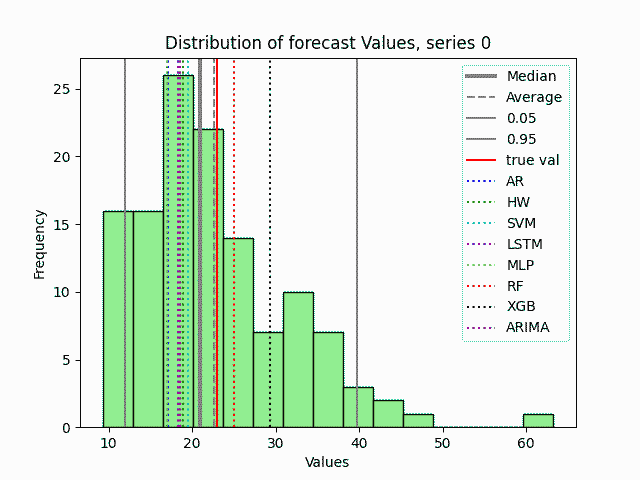
\includegraphics[width=\linewidth]{figs/distr_75_0.png}
		\label{fig:dista}%
		\vspace{0.5em}
		\textit{(a) 75 bootset}
	\end{minipage}
	\hfill
	\begin{minipage}{0.49\textwidth}
		\centering
		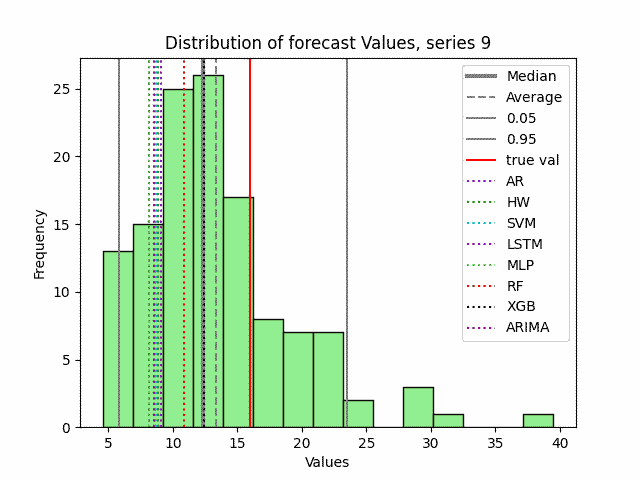
\includegraphics[width=\linewidth]{figs/distr_75_9.png}
		\label{fig:distb}%
		\vspace{0.5em}
		\textit{(b) 125 boostset}
	\end{minipage}
	\caption{Distribution of bootstrap forecasts.}
	\label{fig:distr}
\end{figure}

The relative merits of the different forecasting approaches are better highlighted by critical difference diagrams based on the non-parametric Friedman test followed by a post-hoc Nemenyi test. These diagrams allow for a visual comparison of performance ranks and indicate whether the differences between classifiers are statistically significant \citep{D06}. In our case, the graphs were generated using the SciKit version \citep{SciKitCD} and plot the average rank across all series for each algorithm along the x-axis. Horizontal bars connect those that could not be considered statistically different.

Figures \ref{fig:ywar75} and \ref{fig:ywar175} show a comparison of the ranks on MAE for the 75 series boostset and on MSE for the 175 series boostset. In both cases, as with all those tested, the accuracy of the boost forecasts is significantly higher than that obtained with alternative models. The tables in \ref{app:errcost} confirm that the comparison yields consistent results across all boostset sizes and cost functions, except for bias. The bias rankings are in fact unrelated to those obtained with the other cost functions. This is because the bias is very small in all cases, less than 1\% of the average of the empirical values, which ensures that all the forecasting models are free of systematic errors on our data and makes the difference in the rankings insignificant.

\begin{figure*}
	\centering
	
\includegraphics[width=0.75\linewidth]{figs/sp_MAE_res_YW_AR_75.eps}%
	\caption{Average ranks for MAE on instance res\_YW\_AR\_75}
	\label{fig:ywar75}
\end{figure*}

\begin{figure*}
	\centering
	
\includegraphics[width=0.75\linewidth]{figs/sp_MSE_res_YW_AR_175.eps}%
	\caption{Average ranks for MSE on instance res\_YW\_AR\_175}
	\label{fig:ywar175}
\end{figure*}

Our relatively short time series require a forecasting approach that can handle both limited data and non-stationarity.  Although sophisticated machine learning models such as recurrent neural networks (RNNs) and gradient boosting machines (GBMs) have become more popular in recent years, they can perform less well when there is limited data available, particularly when the data has non-stationary properties. This can lead to overfitting. The autoregressive (AR) model combined with MEB offers a powerful and promising alternative.  This technique performed excellently in the context of this study, consistently outperforming more complex machine learning models. It offers an approach based on robust statistical principles that mitigates the risk of overfitting inherent in many AI approaches. Moreover, the AR model combined with the bootstrap methodology provides reliable forecasts ideally suited to integration into the subsequent optimization module.  

In our case, the choice of an autoregressive (AR) model not only offers superior accuracy, but also several crucial advantages over more complex machine learning approaches. Firstly, the AR model's inherent simplicity makes it easy to implement and interpret.  Unlike many machine learning algorithms, which operate as 'black boxes', the parameters of the AR model have clear statistical interpretations that provide insight into the underlying dynamics of the time series data. Secondly, the well-established theoretical framework of the AR model and the readily available diagnostic tools allow for robust validation and assessment of model performance.  

\subsection{Prescriptive module tests}  \label{Subsec:prescriptive}

The bootstrap forecasts results reported in section \ref{Subsec:predictive} provided the basis for instantiating the optimization phase. The prescriptive module was first run in a deterministic setting, to define a benchmark solution, then extended to the stochastic setting described in section \ref{Sec:optimization}.

When the problem is modelled using the (FD) formulation and the average predictions obtained by boosting are used as deterministic data, it can be easily solved by any state-of-the-art MILP solver. This demonstrates the feasibility of dealing with a significant deterministic equivalent of the stochastic formulation (FS). The optimal deterministic value of $z_{FP} =$ 15553 is used as a benchmark in the following tests.
We moved on to the (DE) formulation generating a value for each of the stochastic variables $\rho_j$ in correspondence to each bootstrap forecast.
%$|S|=100$ scenarios by randomly sampling the stochastic variables $\rho_j$ over the associated probability distributions of the values resulting from the forecasts on all series that are part of a boostset. 
Given these input data, we ran experiments to assess the impact of the variation of the remaining sets of parameters of the formulation, i.e., cardinality of the boostsets, number of splittable clients, and assumptions on inventory costs. 

All reported tests were run on the same machine as in subsection \ref{Subsec:predictive}, a Windows PC workstation equipped with four Intel Core i7-4790 CPUs running at 3.60 GHz and 32 GB of RAM, but in this case the implementation language was C++ to allow finer control over the MILP solver used, which was CPLEX v. 22.11.
These test reports on the sensitivity of the solution to variations in the instance coefficients. Appendix B of the Electronic Companion provides an initial study of the fitness landscape for the split-assignment problem, using a set of artificial benchmark instances.

\subsubsection*{Increasing boostset size}

The size of the boostset helps to stabilize the results during forecasting, as introduced in subsection \ref{Subsec:ambiguity}, but it also has a deep impact on the optimization. In fact, the number of variables and constraints in the DE formulation do not depend on the size of the boostset, larger boostsets are more likely to contain unusual values or combinations thereof. This makes the constraints in equation (\ref{DErequest}) progressively harder to satisfy, which increases the cost and may render the instance infeasible.
To ascertain this, we conducted experiments using 75, 125 and 175 series boostsets, with a time limit of 600 seconds on the optimization process. Figure \ref{fig:bsize} shows a boxplot diagram depicting the distribution of the optimized cost over a number of tests equal to 1/5 of the number of series in the boostset, i.e., 15, 25, 35, respectively.

\begin{figure*}
	\centering
	
\includegraphics[width=0.7\linewidth]{figs/figb0.eps}%
	\caption{Allocation cost for increasing boostset size}
	\label{fig:bsize}
\end{figure*}

Figure \ref{fig:bsize} has a red horizontal line at the cost value for the deterministic case. Therefore, the increase in cost can be considered a quantification of the value of information about storage requests. We observe that the cost remains relatively stable for the 75 and 125 series sets, but increases significantly for the 175 boostset. This is due to the increased difficulty of the larger boostset instances, which meant that some could only be solved heuristically within the time limit. While all instances were feasible, seven out of 35 still had a gap between the lower and upper bounds after 600 seconds of CPU time. 

Finally, we note that, as expected, taking the optimal solution obtained with the coefficients imposed by the 75 series and evaluating it with the coefficients of the 125 series results in a more costly solution than that computed with the 125 series coefficients. More interestingly, however, this solution is not feasible with the 175 series coefficients.

\subsubsection*{Increasing number of splittable clients}

A defining feature of the problem we face is the possibility of accepting split service for some clients. This is unusual for allocation problems and results from the requirement to perform specific what-if analyses on the results. The number of clients allowed to split, and which ones they are, is given in input. In the actual case, the service to a client, if splittable, could be split between at most two servers, and the quantities delivered had to be integers, as specified in all formulations.

The clients to be split are chosen from the most requesting clients. We ran a series of tests based on 75 series boostsets, allowing the 0, 4, 8, and 12 most requesting clients to be split. Figure \ref{fig:bmult} shows the corresponding boxplots.

\begin{figure*}
	\centering
	
\includegraphics[width=0.65\linewidth]{figs/figbmult.eps}%
	\caption{Allocation cost for increasing number of splittable clients}
	\label{fig:bmult}
\end{figure*}

Allowing a service to be split for a client is a partial relaxation of the corresponding assignment constraint, so the expected optimal cost is lower. This can indeed be seen in figure \ref{fig:bmult}, where the more clients that are permitted to split, the lower all distribution moments become. However, the marginal decrease becomes smaller as the number of clients who can split increases, since splitting a small client may result in only a small contribution, if any.

\subsubsection*{Impact of different inventory cost assumptions}

A further set of tests was conducted to determine the impact of inventory costs $d_i$, $i \in I$ on the search process. Recall that in the original case study, one of the objectives was to determine how much space should be rented in the only DC not owned by the company, where storage space needs to be leased. The data of the case study proposed in \citet{MZ23} did not report storage costs. Here, we consider storage costs that are inversely proportional to the average distance of the DC from the stores. We consider three settings, one with no storage costs, one where only the most distant DC incurs costs, and one where all DCs need to lease space. Costs are proportional to the quantities stored and are therefore influenced by the allocation policy.

All the tests were performed using the 75-series boost set. The focus of the analysis is not on the increase in optimal costs, since an increase in the costs of the decision variables clearly leads to an increase in the total costs. Rather, the focus is on the variation in the complexity of the search, as reflected in the CPU time required to reach the final result, and on the optimality or feasibility of the solutions. To evaluate the effectiveness of increasingly lengthy searches, we present results after 600, 1200, and 3600 seconds of CPU time.
The results are summarized in the table \ref{table:qcost}. All results are based on 15 repetitions, and the columns show:
	 $n$: number of clients (stores);
	 $m$: number of servers (DCs);
	 $n_{boost}$: number of series in the boostset;
	 $n_q$: number of servers incurring leasing costs;
	 $n_{inf}$: number of infeasible solutions at the end of the search;
	 {\it GAP lin}: average gap between the linear bound and the best solution at the end of the search;
	 {\it GAP fin}: average gap between the best lower bound and the best solution at the end of the search;
	 {\it t.CPU}: average CPU time (in sec) of the search process.
\begingroup
\renewcommand{\arraystretch}{0.50}
\begin{table}
	\centering
	\renewcommand{\arraystretch}{0.8}
	\begin{tabularx}{0.8\textwidth}{CCCC|CCCC}
		$n$ & $m$ & $n_{boost}$ & $n_q$ & $n_{inf}$ & GAP~lin & GAP~fin & t.CPU \\
		\hline
		52 & 4 & 75        & 0 & 0    & 0.01    & 0.00    &  333.95 \\
		\hline
		52 & 4 & 75        & 1 & 1    & 0.18    & 0.17    &   600  \\
		52 & 4 & 75        & 1 & 0    & 0.15    & 0.14    &  1200 \\
		52 & 4 & 75        & 1 & 0    & 0.14    & 0.13    &  3600 \\
		\hline
		52 & 4 & 75        & 2 & 0    & 0.04    & 0.04    &   600 \\
		52 & 4 & 75        & 2 & 0    & 0.01    & 0.03    &   1200 \\
		52 & 4 & 75        & 2 & 0    & 0.01    & 0.03    &   3600 \\
		\hline
		52 & 4 & 75        & 3 & 0    & 0.01    & 0.00    &  211.03 \\
		\hline
		52 & 4 & 75        & 4 & 0    & 0.01    & 0.00    &  13.00 \\
		\hline
	\end{tabularx}
	\caption{Gap and CPU time for increasing number of leased servers.}
	\label{table:qcost}
\end{table}
\endgroup

Table \ref{table:qcost} illustrates an interesting feature of the fitness landscape of this split-cost allocation problem: the complexity of the search is not monotonic with respect to the number of leased servers. In fact, CPLEX was able to solve all instances to optimality for 0, 3 and 4 leased servers. However, for 1 or 2 leased servers, it was never able to prove the optimality of the best solution found within the time limit of 3600 seconds. Furthermore, instances with one leased server are more challenging than those with two, as demonstrated by the gap between the lower and upper bounds, both between the linear relaxation bound and the best solution found and between the best final lower bound and the best solution. This feature is discussed further in Appendix B of the Electronic Companion.

As a final note, we point out that the objective function was structured to lexicographically first strive for feasibility and then optimize within the feasible domain. In fact, all instances have always resulted in feasible solutions. Reducing the cost coefficient of the request slack variables allows us to explore the trade-off between solution cost and the probability of reaching an infeasible solution. However, we did not explore this further.

\subsubsection*{Test case solution}

To further evaluate the benefits of the proposed approach, we compared the effectiveness of the robust, BESO-optimized solution with that obtained using a parametric method which assumed a Gaussian distribution of forecasts from the request datasets. This comparison was conducted using scenarios derived from a Gaussian distribution based on the confidence intervals of the forecasts provided by an Holt-Winters ETS model \citep{HKOS08}.

Figure \ref{fig:compDistr75} shows the distributions of the forecasts of the 75 boostset obtained by BESO and by ETS. Note that the BESO distribution, given its MEB foundation, spans a wider range of values than the ETS distribution.
The wider distribution has an impact on the proposed allocation. We had empirical proof of this when we tested the BESO and ETS solutions on the validation data obtained by the end of the year.
% — i.e. when we finally received the data for which we were asked to provide a forecast.

\begin{figure*}
	\centering
	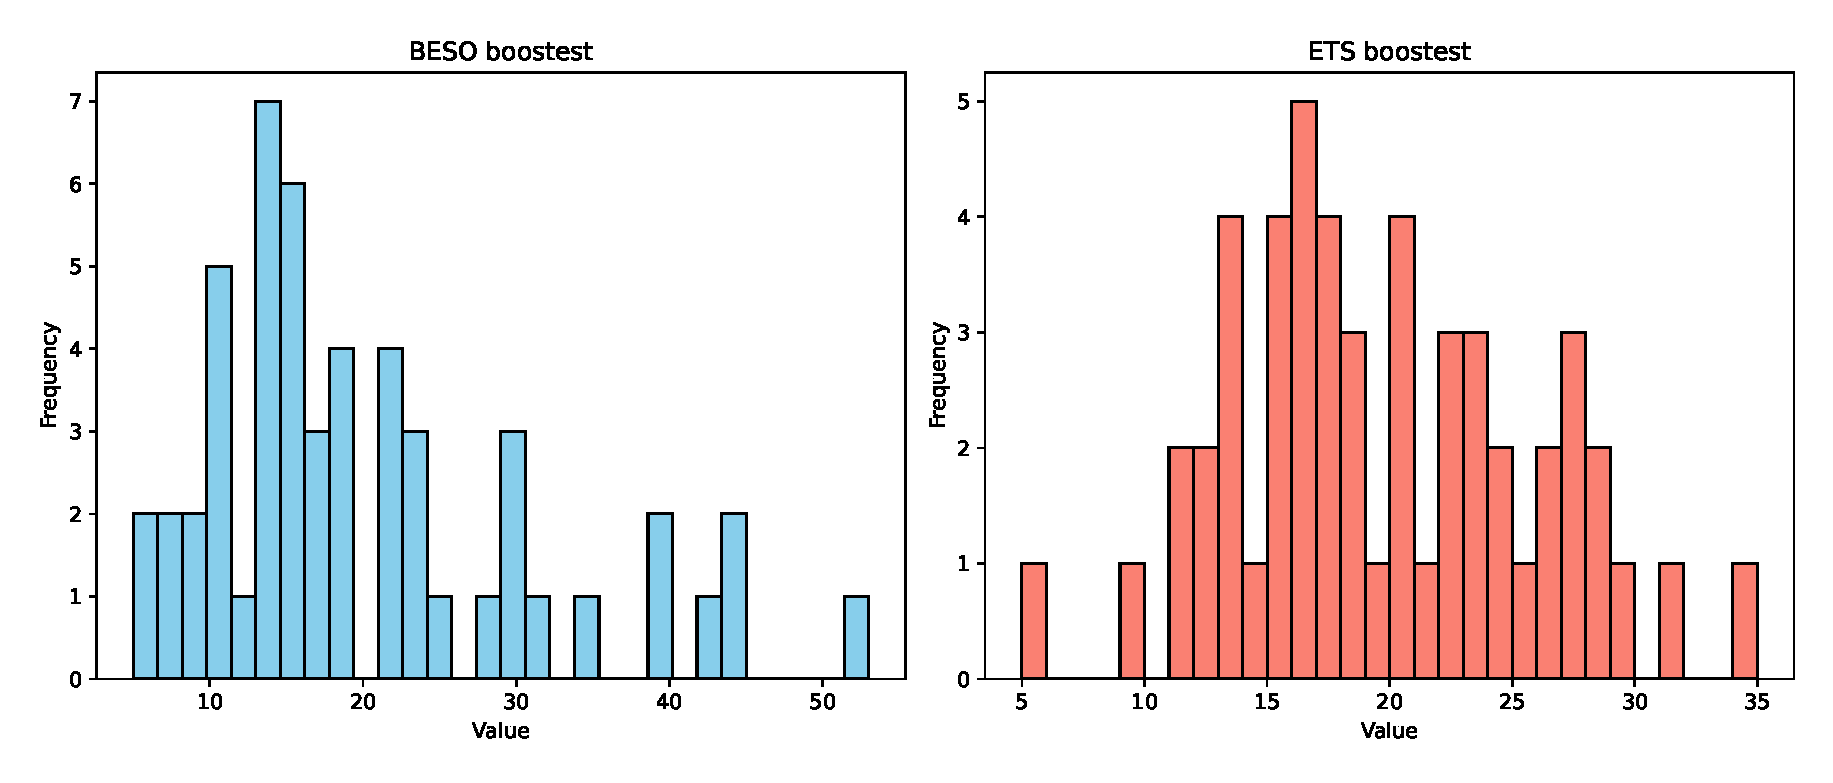
\includegraphics[width=0.75\linewidth]{figs/compDistr.eps}%
	\caption{Comparison of distributions on 75 bootstrapped series}
	\label{fig:compDistr75}
\end{figure*}

Table \ref{table:compETS} presents a comparison of solutions in the first two columns when no rental cost was added for the use of leased floor space and in the last two columns when the rental cost was included in the objective function. As expected, given that the constraints were less restrictive, the ETS solution is less expensive in both cases. However, in both cases, the solution was infeasible as it did not provide all the goods requested by one of the retailers. This result was obtained in a single instance; therefore, it may not have happened. However, it is significant that, even in the first instance in which we tested our model, its robustness proved important in dealing with a limit case.

\begingroup
\renewcommand{\arraystretch}{0.70}
\begin{table}
	\centering
	\begin{tabular}{l|cc|cc|}
		& \multicolumn{2}{|c|}{No rental cost} & \multicolumn{2}{|c|}{With rental cost} \\
		& BESO  & ETS   & BESO    & ETS     \\
		\hline
		Assign. Cost     & 17781 & 15423 & 5446720 & 4378380 \\
		Optimality gap\% & 0     & 0     & 16.07   & 0.69    \\
		Infeasibilities  & 0     & 1     & 0       & 1       \\
		t.Cpu            & 33    & 29    & 3600    & 3600    \\
		\hline
	\end{tabular}
	\caption{Solution cost with and without rental cost}
	\label{table:compETS}
\end{table}
\endgroup

Table \ref{table:resETS} details the proposed usage of the  DCs in the different cases. It appears that DC 2, the biggest owned one, is the overloaded one in both cases, even though by small amounts. 

\begingroup
\renewcommand{\arraystretch}{0.70}
\begin{table}
	\centering
	\begin{tabular}{l|cc|cc|}
		& \multicolumn{2}{|c|}{No rental cost} & \multicolumn{2}{|c|}{With rental cost} \\
		& BESO  & ETS   & BESO    & ETS     \\
		\hline
		DC 0 & 67 / 120 & 119 / 120 & 82 / 120 & 116 / 120 \\
		DC 1 & 571 / 1000 & 430 / 1000 & 532 / 1000 & 428 / 1000 \\
		DC 2 & 257 / 300 & 301 / 300 & 257 / 300 & 303 / 300 \\
		DC 3 & 128 / 180 & 173 / 180 & 152 / 180 & 176 / 180 \\
		\hline
	\end{tabular}
	\caption{DC usage with and without rental cost}
	\label{table:resETS}
\end{table}
\endgroup

Finally, we note that Table \ref{table:compETS} shows that including the rental cost makes otherwise identical instances much harder to solve. In fact, the time limit of 3600 CPU seconds was too short to reach optimality, and a duality gap was left in the proposed solutions, a substantial one in the case of the BESO instance.

\section{Conclusions and future directions} \label{Sec:conclusions}

This paper introduces Bootstrap Enhanced Scenario Optimization (BESO), a framework for deriving predictive prescriptions from  relevant data series. It integrates statistically grounded forecasting with scenario-based optimization by generating future scenarios via bootstrapped autoregressive time series, while incorporating feedback from the optimization stage. A two-echelon logistics case study illustrates how BESO forecasts retailer demand and supports DC allocation, enabling decisions on inventory, capacity, and assignment that reflect both cost structures and uncertainty.

A central contribution of BESO is providing a credible alternative to traditional Distributionally Robust Optimization (DRO). Standard DRO methods rely on predefined ambiguity sets (e.g., moment bounds, Wasserstein metrics, $\phi$-divergences), which may fail to capture complex empirical features such as nonstationarity or heavy tails. BESO instead constructs empirical scenario distributions via Maximum Entropy Bootstrap (MEB), avoiding explicit ambiguity sets. It also allows an objective-aware extension, where optimization-related costs inform the resampling process, producing scenarios aligned with decision quality. The bootstrap size further acts as a transparent control over robustness, replacing exogenous parametric design.

Experiments on real and synthetic data show that BESO yields robust, interpretable prescriptions and adapts well to varying uncertainty structures, achieving performance comparable to classical scenario generation and DRO approaches. Overall, integrating forecasting and optimization within a unified empirical loop enhances both stability and operational effectiveness.

Future research may further explore bootstrap-based ambiguity representations, positioning BESO as a data-driven DRO alternative. Extensions could include hybrid schemes incorporating prior knowledge or Bayesian elements, as well as broader applicability to settings where reliable forecasting models are not available.

% References 
\bibliographystyle{informs2014} % outcomment this and next line in Case 1
\bibliography{GDObiblio} % if more than one, comma separated

%%%%%%%%%%%%%%%%%
\end{document}
%%%%%%%%%%%%%%%%%



